\documentclass[12pt]{extarticle}
\usepackage{import}
\import{./}{Includes}

\begin{document}
\atitle{3}
 
\section*{Problem 1.}
Let $(X, \topo)$ be a topological space and $f : X \rightarrow Y$ be any function. Define \[\mathcal{S} = \{ U \in \bf{P}\left(Y\right) \mid \invI{f}{U} \in \topo \}\]
Since $\invI{f}{Y} = X$ and $\invI{f}{\emptyset} = \emptyset$ then $\emptyset, Y \in \mathcal{S}$. \\ \smallskip
Suppose that for some index set $\Lambda$, the sets $V_\lambda \in \mathcal{S}$. Then by Lemma \ref{invunion}, \[\invI{f}{\bigcup_{\lambda \in \Lambda} V_\lambda} = \bigcup_{\lambda \in \Lambda} \invI{f}{V_\lambda} \in \topo\]
Because each $V_\lambda \in \topo$ and $\topo$ is closed under arbitrary unions. Therefore, $\bigcup\limits_{\lambda \in \Lambda} V_\lambda \in \mathcal{S}$. \\
Suppose that for some \emph{finite} index set $\Lambda$, the sets $V_\lambda \in \mathcal{S}$. Then by Lemma \ref{invunion}, \[\invI{f}{\bigcap_{\lambda \in \Lambda} V_\lambda} = \bigcap_{\lambda \in \Lambda} \invI{f}{V_\lambda} \in \topo\]
Because each $V_\lambda \in \topo$ and $\topo$ is closed under finite intersections. Therefore, $\bigcap\limits_{\lambda \in \Lambda} V_\lambda \in \mathcal{S}$. \\
Thus, $\mathcal{S}$ is a topology on $Y$. 

\section*{Problem 2.}
The basis $\base = \{V \times W \mid V \in \topo_Y \text{ and } W \in \topo_W \}$ generates the product topology $\topo_{Y \times Z}$ on the space $Y \times Z$. Thus by Lemma \ref{baisunion}, the open sets in $\topo_{Y \times Z}$ are exactly those that are unions of basis elements. Therefore, \[U \in \topo_{Y \times Z} \iff U = \bigcup\limits_{\lambda \in \Lambda} V_\lambda \times W_\lambda\] 
with $V_\lambda \times W_\lambda \in \base$ i.e. for $V_\lambda \in \topo_Y$ and $W_\lambda \in \topo_Z$.

\section*{Problem 3.}
Let $X$, $Y$, and $Z$ be topological spaces and $Y \times Z$ have the product topology. Suppose that $f_1 : X \rightarrow Y$ and $f_2 : X \rightarrow Z$ are continuous. Then define $F : X \rightarrow Y \times Z$ by $F : x \mapsto (f_1(x), f_2(x))$. Take $U$ open in $\topo_{Y \times Z}$ so, by problem 2, $U = \bigcup\limits_{\lambda \in \Lambda} V_\lambda \times W_\lambda$ with $V_\lambda \in \topo_Y$ and $W_\lambda \in \topo_Z$. Then, 
\begin{align*}
x \in \invI{F}{U} & \iff (f_1(x), f_2(x)) \in \bigcup\limits_{\lambda \in \Lambda} V_\lambda \times W_\lambda \iff \exists \lambda \in \Lambda : f_1(x) \in V_\lambda \text{ and } f_2(x) \in W_\lambda \\ & \iff \exists \lambda \in \Lambda : x \in \invI{f_1}{V_\lambda} \cap \invI{f_2}{W_\lambda} \iff x \in \bigcup_{\lambda \in \Lambda} \invI{f_1}{V_\lambda} \cap \invI{f_2}{W_\lambda}  
\end{align*}
Thus, \[\invI{F}{U} = \bigcup\limits_{\lambda \in \Lambda} \invI{f_1}{V_\lambda} \cap \invI{f_2}{W_\lambda}\]
Now by continuity of $f_1$ and $f_2$, the sets $\invI{f_1}{V_\lambda}$ and $\invI{f_2}{W_\lambda}$ are open in $X$ and since $X$ is a topological space, their intersection is open.
Therefore, \[\invI{F}{U} = \bigcup\limits_{\lambda \in \Lambda} \invI{f_1}{V_\lambda} \cap \invI{f_2}{W_\lambda} \in \topo_X\] because it is a union of open sets of $X$ which shows that $F$ is continuous.
\bigskip \\
Now let one of $f_1$ and $f_2$ be not continuous. WLOG take $f_1$ to be not continous. Then for some $V \in \topo_Y$, we must have $\invI{f_1}{V} \notin \topo_X$. Then $V \times Z \in \topo_{Y \times Z}$ because $Z \in \topo_Z$. Consider, \[x \in \invI{F}{V \times Z} \iff (f_1(x), f_2(x)) \in V \times Z \iff f_1(x) \in V\]
Because for any $x$, $f_2(x) \in Z$. Thus, $\invI{F}{V \times Z} = \invI{f_1}{V} \notin \topo_X$ so $F$ cannot be continuous. 

\section*{Problem 4.}
\begin{enumerate}
\item The function $\log : \Rplus \rightarrow \R$ is continuous by its integral definition (since the subspace topology on $\Rplus$ is generated by the same metric that generates the standard topology on $\R$). Furthermore, $\log$ has an inverse namely $\exp$ which is also continuous because it is differentiable. Thus, $\log$ is a homeomorphism between $\Rplus$ and $\R$. 

\item  Let \[S = \{(x, y) \in \R^2 \mid x^2 + y^2 = 1\}\]
Define $F : \R^2 \sm \{(0,0)\} \rightarrow \R \times S$ by $F : (x, y) \mapsto \left(\log{\sqrt{x^2 + y^2}}, \left(\frac{x}{\sqrt{x^2 + y^2}}, \frac{y}{\sqrt{x^2 + y^2}} \right) \right)$ \\

Now the functions $f_1 : \R^2 \sm \{(0,0)\} \rightarrow \R$ and $f_2 : \R^2 \sm \{(0,0)\} \rightarrow S$ given by \[f_1 : (x, y) \mapsto \log{\sqrt{x^2+y^2}} \text{ and } f_2 : (x,y) \mapsto \left(\frac{x}{\sqrt{x^2 + y^2}}, \frac{y}{\sqrt{x^2 + y^2}} \right)\] are continous by $\epsilon, \delta$ arguments. Then $F = (f_1, f_2)$ so by problem 3, $F$ is continuous under the product topology on $\R \times S$. \bigskip \\ Now define $G : \R \times S \rightarrow \R^2 \sm \{(0,0)\}$ by $G : (r, (x, y)) \mapsto (x e^r, y e^r)$. Thus, \[F \circ G(r, (x, y)) = F(x e^r, y e^r) = \left(\log{e^r \sqrt{x^2 + y^2}}, \left(\frac{x e^r}{e^r \sqrt{x^2 + y^2}}, \frac{y e^r}{e^r \sqrt{x^2 + y^2}} \right) \right)\]
But $(x, y) \in S$ so $x^2 + y^2 = 1$ and $e^r > 0$ thus, $F \circ G(r, (x, y)) = (r, (x, y))$. \\
Furthermore, for $(x,y) \neq (0,0)$ (such that $F(x,y)$ is defined) we have,
\begin{align*}
G \circ F(x, y) &= G \left(\log{\sqrt{x^2 + y^2}}, \left(\frac{x}{\sqrt{x^2 + y^2}}, \frac{y}{\sqrt{x^2 + y^2}} \right) \right) \\ &= \left(\frac{x}{\sqrt{x^2 + y^2}} \exp{\log{\sqrt{x^2 + y^2}}}, \frac{y}{\sqrt{x^2 + y^2}} \exp{\log{\sqrt{x^2 + y^2}}}  \right)  = (x, y)
\end{align*}

Therefore, $G \circ F = \mathrm{id}_{\R^2 \setminus \{(0,0)\}}$ and $F \circ G = \mathrm{id}_{\R \times S}$ so, in particular, $F$ is a bijection. Since the product topology on $\R \times S$ is metrizable by the $\R^3$ Euclidean metric, we can use standard analysis facts to conculde that $G$ extended to $\R^3 \rightarrow \R^2 \sm \{(0,0)\}$ is continuous with respect to the Euclidean metric thus its restriction to $\R \times S$ is also continuous.    

\end{enumerate}

\section*{Problem 5.}
For $\bf{u}, \bf{v} \in \R^2$ define:
\[ d(\bf{u}, \bf{v}) =  \begin{cases} |\bf{u} - \bf{v}| & \text{ if } \bf{u} = t\bf{v} \text{ for } t \in \R \\ |\bf{u} | + |\bf{v}| & \text{ otherwise} \end{cases}\]
Since both $|\bf{u} - \bf{v}| \ge 0$ and $|\bf{u}| + |\bf{v}| \ge 0$ then $d(\bf{u}, \bf{v}) \ge 0$. \\ 
Since both $|\bf{u} - \bf{v}|  = |\bf{v} - \bf{u}|$ and $|\bf{u}| + |\bf{v}| = |\bf{v}| + |\bf{u}|$ then $d(\bf{u}, \bf{v}) = d(\bf{v}, \bf{u})$. \\   
Also $|\bf{u} - \bf{v}| = 0 \iff \bf{u} = \bf{v}$ and $|\bf{u}| + |\bf{v}| = 0 \iff |\bf{u} | = |\bf{v}| = 0 \iff \bf{u} = \bf{v} = 0$ then $d(\bf{u}, \bf{v}) = 0 \iff \bf{u} = \bf{v}$. \\\\
Then take any $\bf{w} \in \R^2$. First, suppose that $\bf{u} = t \bf{v}$ for $t \in \R$ so $d(\bf{u}, \bf{v}) = |\bf{u} - \bf{v}|$. Then by the triangle inequality for the Euclidean norm, \[|\bf{u} - \bf{v}| =  |\bf{u} - \bf{w} + \bf{w} - \bf{v}| \le |\bf{u} - \bf{w} | + |\bf{w} - \bf{v}| \le (|\bf{u}| + |\bf{w}|) + (|\bf{w}| + |\bf{v}|)\] 
Therefore $d(\bf{u}, \bf{v}) \le d(\bf{u}, \bf{w}) + d(\bf{w}, \bf{v})$ because $|\bf{u} - \bf{w}| \le d(\bf{u}, \bf{w})$. \\\\
Otherwise, it cannot be that $\bf{u} = t \bf{w}$ and $\bf{w} = t'\bf{v}$ else $\bf{u} = t \cdot t'\bf{v}$. \\
If $\bf{w}$ is not a multiple of either $\bf{u}$ or $\bf{v}$ then,
\[d(\bf{u}, \bf{v})  = |\bf{u}| + |\bf{v}| \le |\bf{u}| + |\bf{w}| + |\bf{w}| + |\bf{v}| = d(\bf{u}, \bf{w}) + d(\bf{w}, \bf{v})\]

If $\bf{w} = t \bf{u}$ then using Lemma \ref{subineq},
\[d(\bf{u}, \bf{v})  = |\bf{u}| + |\bf{v}| = |\bf{u}| - |\bf{w}| + |\bf{w}| + |\bf{v}| \le |\bf{u} - \bf{w} | + |\bf{w}| + |\bf{v}| = d(\bf{u}, \bf{w}) + d(\bf{w}, \bf{v})\] 

If $\bf{w} = t \bf{v}$ then using Lemma \ref{subineq},
\[d(\bf{u}, \bf{v})  = |\bf{u}| + |\bf{v}| = |\bf{u}| + |\bf{w}| + |\bf{v}| - |\bf{w}| \le |\bf{u}| + | \bf{w} | + |\bf{v} - \bf{w}| = d(\bf{u}, \bf{w}) + d(\bf{v}, \bf{w})\] 
Therefore, for all vectors, $d(\bf{u}, \bf{v}) \le d(\bf{u}, \bf{w}) + d(\bf{w}, \bf{v})$ so $d$ is a metric. \\ \\

However, $d$ does not generate the standard topology on $\R^2$. Consider \[\ball{\frac{1}{2}}{(1, 0)}^{\text{Rail}} = \{(x, 0) \mid x \in \left(\tfrac{1}{2}, \tfrac{3}{2} \right) \}\]
This equality holds because if $\bf{v} \neq (x, 0) = x \cdot (1, 0)$ then $d(\bf{v}, (1, 0)) = |\bf{v}| + |(1,0)| \ge 1$. \bigskip \\
Now, suppose $\exists \delta \in \Rplus : \ball{\delta}{(1,0)}^{\text{Std.}} \subset \ball{\delta}{(1,0)}^{\text{Rail}}$ then  \bigskip $(1, \delta) \in \ball{\delta}{(1,0)}^{\text{Std.}} \subset \ball{\delta}{(1,0)}^{\text{Rail}}$ which is a contradiction. \bigskip Thus, $\ball{\frac{1}{2}}{(1, 0)}^{\text{Rail}}$ is not an open set of the standard topology but it is by definition open in the topology generated by this new metric.  

\section*{Problem 6.}

\begin{enumerate}
\item
Let $X = \{a, b \}$ and $\topo = \{\{a \}, \{a,b\}, \emptyset \}$. Suppose a metric $d$ generates $\topo$. Then let $\delta = d(a,b)$ then $b \in \ball{\delta}{b}$ but $a \notin \ball{\delta}{b}$ because $d(a, b) \not\le \delta = d(a,b)$. Thus $\ball{\delta}{a} \notin \topo$. Thus, $\topo$ cannot be generated by the metric $d$.

\item Let $X$ be a finite set and $d$ be a metric on $X$. Consider $x \in X$ and define \[\delta_x = \min\limits_{y \in X \sm \{x\}} d(x,y)\] which exists and is positive because each $d(x, y) > 0$. Then $x \in \ball{\delta_x}{x}$ but for any other $y \in X$ s.t. $x \neq y$, we have $y \notin \ball{\delta_x}{x}$ because \[\delta_x = \min\limits_{y \in X \setminus \{x\}} d(x,y) < d(x,y)\] So $\ball{\delta_x}{x} = \{x\}$ is open in the topology generated by $d$. For any $S \subset X$, $S = \bigcup\limits_{x \in S} \{x\}$ is open because each $\{x\}$ is open. Thus, any metric on $X$ generates the discrete topology. 

\end{enumerate}

\section*{Problem 7.} For $\bf{u}, \bf{v} \in \R^n$ define:
\[d'(\bf{u}, \bf{v}) = \sum\limits_{i = 1}^{n} |u_i - v_i|\]

Then each $|u_i - v_i| \ge 0$ so we get $d'(\bf{u}, \bf{v}) \ge 0$. Also each $|u_i - v_i| = |v_i - u_i|$ so $d'(\bf{u}, \bf{v}) = d'(\bf{v}, \bf{u})$.
Also, $d'(\bf{u}, \bf{v}) = 0 \iff \forall i \in \{1, \dots, n\} : |u_i - v_i| = 0 \iff u_i = v_i \iff \bf{u} = \bf{v}$.
Now, \[d'(\bf{u}, \bf{v}) = \sum\limits_{i = 1}^{n} |u_i - v_i| = \sum\limits_{i = 1}^{n} |u_i - w_i + w_i - v_i| \le \sum\limits_{i = 1}^{n} |u_i - w_i| + \sum\limits_{i = 1}^{n} |w_i - v_i| = d'(\bf{u}, \bf{w}) + d'(\bf{w}, \bf{v}) \]
by the triangle inequality for the absolute value function. Thus, $d'$ is a metric. \bigskip \\ It remains to be shown that this metric generates the standard topology on $\R^n$. Using the notation $\ball{\delta}{\bf{x}}' = \{ \bf{y} \in \R^n \mid d'(\bf{x}, \bf{y}) < \delta\}$, I claim that $\ball{\frac{\delta}{n}}{\bf{x}} \subset \ball{\delta}{\bf{x}}' \subset \ball{\delta}{\bf{x}}$ because:
\begin{align*}
\bf{y} \in \ball{\frac{\delta}{n}}{\bf{x}} & \implies d(\bf{x}, \bf{y}) = |\bf{x} - \bf{y}| < \delta/n \implies |x_i - y_i| \le |\bf{x} - \bf{y}| < \delta/n \\ & \implies d'(\bf{x}, \bf{y}) = \sum\limits_{i = 1}^{n} |x_i - y_i| < \delta \implies \bf{y} \in \ball{\delta}{\bf{x}}
\end{align*}
Furthermore, because 
\[d'(\bf{x}, \bf{y})^2 = \left( \sum\limits_{i = 1}^{n} |x_i - y_i| \right)^2 = \sum\limits_{i = 1}^{n} |x_i - y_i|^2  + \sum\limits_{i \neq j} |x_i - y_i| |x_j - y_j| \ge \sum\limits_{i = 1}^{n} |x_i - y_i|^2 \]
we have
\begin{align*}
\bf{y} \in \ball{\delta}{\bf{x}}' & \implies d'(\bf{x}, \bf{y}) < \delta \implies d(\bf{x}, \bf{y}) = \sqrt{\sum\limits_{i = 1}^{n} |x_i - y_i|^2} \le \sum\limits_{i = 1}^{n} |x_i - y_i| < \delta \implies \bf{x} \in \ball{\delta}{\bf{x}}
\end{align*}

Suppose that $U \in \topo_{d}$ then $\forall \bf{x} \in U : \exists \delta > 0 : x \in \ball{\delta}{\bf{x}} \subset U$ thus $\bf{x} \in \ball{\delta}{\bf{x}}' \subset \ball{\delta}{\bf{x}} \subset U$ so $\exists \delta > 0 : \bf{x} \in \ball{\delta}{\bf{x}}' \subset U$ thus $U \in \topo_{d'}$. \bigskip \\
Conversely, if $U \in \topo_{d'}$ then $\forall \bf{x} \in U : \exists \delta > 0 : \bf{x} \in \ball{\delta}{\bf{x}}' \subset U$ thus $\bf{x} \in \ball{\frac{\delta}{n}}{\bf{x}} \subset \ball{\bf{x}}{\delta}' \subset U$ so $\exists \tilde{\delta} = \delta/n > 0 : \bf{x} \in \ball{\tilde{\delta}}{\bf{x}} \subset U$ thus $U \in \topo_{d}$. Therefore, $\topo_{d} = \topo_{d'}$.  

\begin{figure}
\center{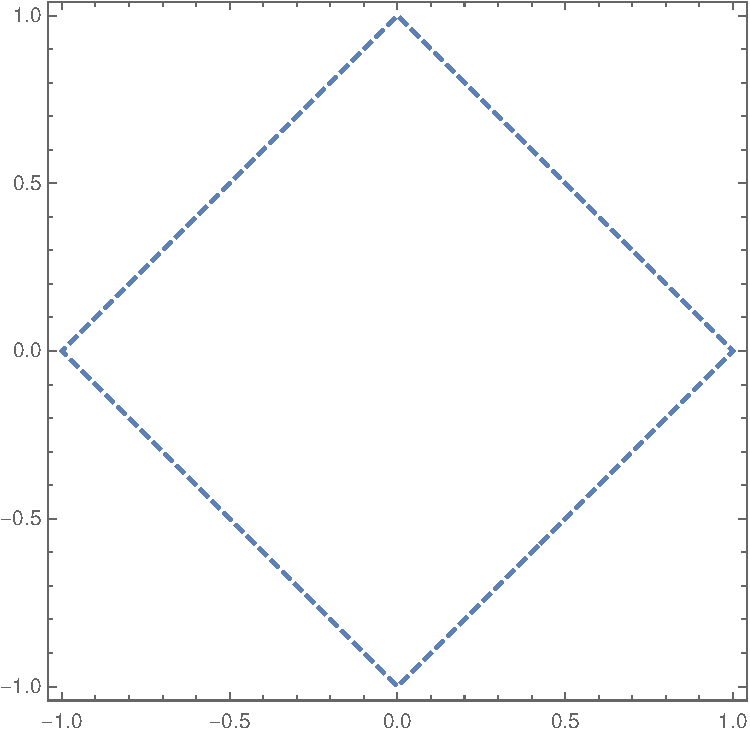
\includegraphics[width=3in]{diamond.pdf}}
\vspace*{-5mm}
\caption{An open "ball" in $\R^2$ under the metric $d'$ with radius $1$ centered at $(0, 0)$}

\label{fig:fourierfluc}
\end{figure}

\section*{Lemmas}

\begin{lemma} \label{invunion}
For any index set $\Lambda$, $\invI{f}{\bigcup\limits_{\lambda \in \Lambda} V_\lambda} = \bigcup\limits_{\lambda \in \Lambda} \invI{f}{V_\lambda}$ and $\invI{f}{\bigcap\limits_{\lambda \in \Lambda} V_\lambda} = \bigcap\limits_{\lambda \in \Lambda} \invI{f}{V_\lambda}$
\end{lemma}
\begin{proof}
\begin{align*}
x \in \invI{f}{\bigcup\limits_{\lambda \in \Lambda} V_\lambda} & \iff f(x) \in \bigcup\limits_{\lambda \in \Lambda} V_\lambda \iff \exists \lambda \in \Lambda : f(x) \in V_\lambda\\ & \iff \exists \lambda \in \Lambda : x \in \invI{f}{V_\lambda} \iff x \in \bigcup\limits_{\lambda \in \Lambda} \invI{f}{V_\lambda}
\end{align*}
Thus, $\invI{f}{\bigcup\limits_{\lambda \in \Lambda} V_\lambda} = \bigcup\limits_{\lambda \in \Lambda} \invI{f}{V_\lambda}$. Also, \\\\
\begin{align*}
x \in \invI{f}{\bigcap\limits_{\lambda \in \Lambda} V_\lambda} & \iff f(x) \in \bigcap\limits_{\lambda \in \Lambda} V_\lambda \iff \exists \lambda \in \Lambda : f(x) \in V_\lambda\\ & \iff \exists \lambda \in \Lambda : x \in \invI{f}{V_\lambda} \iff x \in \bigcup\limits_{\lambda \in \Lambda} \invI{f}{V_\lambda}
\end{align*}
Thus, $\invI{f}{\bigcup\limits_{\lambda \in \Lambda} V_\lambda} = \bigcup\limits_{\lambda \in \Lambda} \invI{f}{V_\lambda}$.
\end{proof}

\begin{lemma} \label{baisunion}
Let the basis $\base$ generate a topology $\topo$ then $U \in \topo \iff U = \bigcup\limits_{\lambda \in \Lambda} B_\lambda$ with $B_\lambda \in \base$
\end{lemma}

\begin{proof}
If $U \in \topo$ then $\forall x \in U : \exists V_x \in \base : x \in B_x \subset U$. Then \[\bigcup\limits_{x \in U} \{x \} \subset \bigcup\limits_{x \in U} B_x \subset U\]
However, $\bigcup\limits_{x \in U} \{x\} = U$ so \[U =  \bigcup\limits_{x \in U} B_x\]
Conversely, each $B_\lambda \in \base$ is open and thus \[U = \bigcup\limits_{\lambda \in \Lambda} B_\lambda \]
is also open because it is the union of open sets.
\end{proof}

\begin{lemma} \label{subineq}
$\big| |\bf{u}| - |\bf{v}| \big| \le |\bf{u} - \bf{v}|$
\end{lemma}

\begin{proof}
By the triangle inequality, \[|\bf{u}| \le |\bf{u} - \bf{v}| + |\bf{v}| \text{ so }|\bf{u}| - |\bf{v}| \le |\bf{u} - \bf{v}|\] Similarly, \[ |\bf{v}| \le |\bf{v} - \bf{u}| + |\bf{u}| \text{ so } |\bf{v}| - |\bf{u}| \le |\bf{v} - \bf{u}|\]
Thus, \[ -|\bf{u} - \bf{v}| \le |\bf{u}| - |\bf{v}| \le |\bf{u} - \bf{v}| \]
So, \[ \big| |\bf{u}| - |\bf{v}| \big| \le |\bf{u} - \bf{v}|\]
\end{proof}

\end{document}